% questions.tex —— 2004 年·全国卷Ⅲ·文科 · 题目内容片段（无答案）
% 由 tools/generate_projects.py 依来源总账自 2004/2004_数学真题_全国3文_试题.md 生成，勿手改（改源 MD 后重跑）


\begin{gktip}
\textbf{来源说明}：本题面依据固定源 PDF 两页 A3 题面逐题转录，原卷印刷页码 192–193。固定源不附答案，答案和解析均由本库独立复算。

\textbf{图形说明}：第 21 题的原卷图形关系重绘为 TikZ/PGFPlots 矢量图。图形标记所指的 PNG 不随仓库保存。
\end{gktip}

\gkpart{一、选择题（本大题共 12 小题，每小题 5 分，共 60 分．在每小题给出的四个选项中，只有一项是符合题目要求的）}

\begin{question}
\gkti{1}设集合 $M=\{(x,y)\mid x^2+y^2=1,x\in\mathbf{R},y\in\mathbf{R}\}$，$N=\{(x,y)\mid x^2-y=0,x\in\mathbf{R},y\in\mathbf{R}\}$，则集合 $M\cap N$ 中元素的个数为\mbox{（　　）}

（A）1　　（B）2　　（C）3　　（D）4

\end{question}
\begin{question}
\gkti{2}函数 $y=\left|\sin\dfrac{x}{2}\right|$ 的最小正周期是\mbox{（　　）}

（A）$\dfrac{\pi}{2}$　　（B）$\pi$　　（C）$2\pi$　　（D）$4\pi$

\end{question}
\begin{question}
\gkti{3}记函数 $y=1+3^{-x}$ 的反函数为 $y=g(x)$，则 $g(10)=$\mbox{（　　）}

（A）2　　（B）$-2$　　（C）3　　（D）$-1$

\end{question}
\begin{question}
\gkti{4}等比数列 $\{a_n\}$ 中，$a_2=9$，$a_5=243$，则 $\{a_n\}$ 的前 4 项和为\mbox{（　　）}

（A）81　　（B）120　　（C）168　　（D）192

\end{question}
\begin{question}
\gkti{5}圆 $x^2+y^2-4x=0$ 在点 $P(1,\sqrt{3})$ 处的切线方程为\mbox{（　　）}

（A）$x+\sqrt{3}y-2=0$　　（B）$x+\sqrt{3}y-4=0$

（C）$x-\sqrt{3}y+4=0$　　（D）$x-\sqrt{3}y+2=0$

\end{question}
\begin{question}
\gkti{6}$\left(\sqrt{x}-\dfrac{1}{x}\right)^6$ 展开式中的常数项为\mbox{（　　）}

（A）15　　（B）$-15$　　（C）20　　（D）$-20$

\end{question}
\begin{question}
\gkti{7}设复数 $z$ 的辐角主值为 $\dfrac{2\pi}{3}$，虚部为 $\sqrt{3}$，则 $z^2=$\mbox{（　　）}

（A）$-2-2\sqrt{3}\mathrm{i}$　　（B）$-2\sqrt{3}-2\mathrm{i}$

（C）$2+2\sqrt{3}\mathrm{i}$　　（D）$2\sqrt{3}+2\mathrm{i}$

\end{question}
\begin{question}
\gkti{8}设双曲线的焦点在 $x$ 轴上，两条渐近线为 $y=\pm\dfrac{1}{2}x$，则该双曲线的离心率 $e=$\mbox{（　　）}

（A）5　　（B）$\sqrt{5}$　　（C）$\dfrac{\sqrt{5}}{2}$　　（D）$\dfrac{\sqrt{5}}{4}$

\end{question}
\begin{question}
\gkti{9}不等式 $1<|x+1|<3$ 的解集为\mbox{（　　）}

（A）$(0,2)$　　（B）$(-2,0)\cup(2,4)$

（C）$(-4,0)$　　（D）$(-4,-2)\cup(0,2)$

\end{question}
\begin{question}
\gkti{10}正三棱锥的底面边长为 2，侧面均为直角三角形，则此三棱锥的体积为\mbox{（　　）}

（A）$\dfrac{2\sqrt{2}}{3}$　　（B）$\sqrt{2}$　　（C）$\dfrac{\sqrt{2}}{3}$　　（D）$\dfrac{4\sqrt{2}}{3}$

\end{question}
\begin{question}
\gkti{11}在 $\triangle ABC$ 中，$AB=3$，$BC=\sqrt{13}$，$AC=4$，则边 $AC$ 上的高为\mbox{（　　）}

（A）$\dfrac{3\sqrt{2}}{2}$　　（B）$\dfrac{3\sqrt{3}}{2}$　　（C）$\dfrac{3}{2}$　　（D）$3\sqrt{3}$

\end{question}
\begin{question}
\gkti{12}将 4 名教师分配到 3 所中学任教，每所中学至少 1 名，则不同的分配方案共有\mbox{（　　）}

（A）12 种　　（B）24 种　　（C）36 种　　（D）48 种

\end{question}
\gkpart{二、填空题（本大题共 4 小题，每小题 4 分，共 16 分．把答案填在横线上）}

\begin{question}
\gkti{13}函数 $y=\sqrt{\log_{\frac{1}{2}}(x-1)}$ 的定义域是 $\underline{\hspace{3cm}}$。

\end{question}
\begin{question}
\gkti{14}用平面 $\alpha$ 截半径为 $R$ 的球，如果球心到平面 $\alpha$ 的距离为 $\dfrac{R}{2}$，那么截得小圆的面积与球的表面积的比值为 $\underline{\hspace{3cm}}$。

\end{question}
\begin{question}
\gkti{15}函数 $y=\sin x-\dfrac{1}{2}\cos x$（$x\in\mathbf{R}$）的最大值为 $\underline{\hspace{3cm}}$。

\end{question}
\begin{question}
\gkti{16}设 $P$ 为圆 $x^2+y^2=1$ 上的动点，则点 $P$ 到直线 $3x-4y-10=0$ 的距离的最小值为 $\underline{\hspace{3cm}}$。

\end{question}
\gkpart{三、解答题（本大题共 6 小题，共 74 分．解答应写出文字说明、证明过程或演算步骤）}

\begin{question}
\gkti{17}（本小题满分 12 分）

解方程：$4^x-2^{x+2}-12=0$。

\end{question}
\begin{question}
\gkti{18}（本小题满分 12 分）

已知 $\alpha$ 为锐角，且 $\tan\alpha=\dfrac{1}{2}$，求 $\dfrac{\sin 2\alpha\cos\alpha-\sin\alpha}{\sin 2\alpha\cos 2\alpha}$ 的值。

\end{question}
\begin{question}
\gkti{19}（本小题满分 12 分）

设数列 $\{a_n\}$ 是公差不为零的等差数列，$S_n$ 是数列 $\{a_n\}$ 的前 $n$ 项和，且 $S_1^2=9S_2$，$S_4=4S_2$，求数列 $\{a_n\}$ 的通项公式。

\end{question}
\begin{question}
\gkti{20}（本小题满分 12 分）

某村计划建造一个室内面积为 $800\text{ m}^2$ 的矩形蔬菜温室。在温室内，沿左、右两侧与后侧内墙各保留 $1\text{ m}$ 宽的通道，沿前侧内墙保留 $3\text{ m}$ 宽的空地。当矩形温室的边长各为多少时，蔬菜的种植面积最大？最大种植面积是多少？

\Needspace{0.4\textheight}
\end{question}
\begin{question}
\gkti{21}（本小题满分 12 分）

三棱锥 $P-ABC$ 中，侧面 $PAC$ 与底面 $ABC$ 垂直，$PA=PB=PC=3$。
\nopagebreak[4]
\begin{center}% 2004 年全国卷Ⅲ文科第 21 题：三棱锥立体几何图
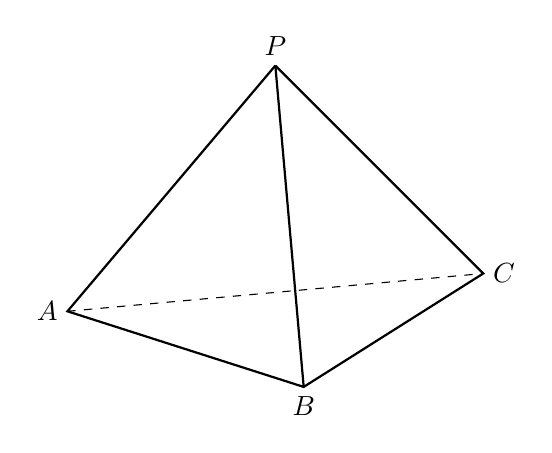
\begin{tikzpicture}[>=stealth,scale=1.2]
  % Coordinates
  \coordinate (A) at (-2.2,-0.4);
  \coordinate (B) at (0.3,-1.2);
  \coordinate (C) at (2.2,0);
  \coordinate (P) at (0,2.2);

  % Edges
  \draw[thick] (P) -- (A) -- (B) -- (C) -- (P);
  \draw[thick] (P) -- (B);
  \draw[dashed] (A) -- (C);

  % Labels
  \node[left] at (A) {$A$};
  \node[below] at (B) {$B$};
  \node[right] at (C) {$C$};
  \node[above] at (P) {$P$};
\end{tikzpicture}
\end{center}
\nopagebreak[4]
（1）求证：$AB\perp BC$；

（2）设 $AB=BC=2\sqrt{3}$，求 $AC$ 与平面 $PBC$ 所成角的大小。

\end{question}
\begin{question}
\gkti{22}（本小题满分 14 分）

设椭圆 $\dfrac{x^2}{m+1}+y^2=1$ 的两个焦点是 $F_1(-c,0)$ 与 $F_2(c,0)$（$c>0$），且椭圆上存在一点 $P$，使得直线 $PF_1$ 与 $PF_2$ 垂直。

（1）求实数 $m$ 的取值范围；

（2）设 $L$ 是相应于焦点 $F_2$ 的准线，直线 $PF_2$ 与 $L$ 相交于点 $Q$，若 $\dfrac{|QF_2|}{|PF_2|}=2-\sqrt{3}$，求直线 $PF_2$ 的方程。

\end{question}